% Template source: University of Florida Department of Physics, https://www.phys.ufl.edu/courses/phy4803L/sample-paper.zip

\documentclass[aps,twocolumn,secnumarabic,nobalancelastpage,amsmath,amssymb,nofootinbib]{revtex4}

% Documentclass Options
    % aps, prl, rmp stand for American Physical Society, Physical Review Letters, and Reviews of Modern Physics, respectively
    % twocolumn permits two columns, of course
    % nobalancelastpage doesn't attempt to equalize the lengths of the two columns on the last page
        % as might be desired in a journal where articles follow one another closely
    % amsmath and amssymb are necessary for the subequations environment among others
    % secnumarabic identifies sections by number to aid electronic review and commentary.
    % nofootinbib forces footnotes to occur on the page where they are first referenced
        % and not in the bibliography
    % REVTeX 4 is a set of macro packages designed to be used with LaTeX 2e.
        % REVTeX is well-suited for preparing manuscripts for submission to APS journals.


\usepackage{chapterbib}    % allows a bibliography for each chapter (each labguide has it's own)
\usepackage{color}         % produces boxes or entire pages with colored backgrounds
\usepackage{graphics}      % standard graphics specifications
\usepackage[pdftex]{graphicx}      % alternative graphics specifications
\usepackage{longtable}     % helps with long table options
\usepackage{epsf}          % old package handles encapsulated post script issues
\usepackage{bm}            % special 'bold-math' package
\usepackage{verbatim}			% for comment environment
\usepackage[colorlinks=true]{hyperref}  % this package should be added after all others
                                        % use as follows: \url{https://urldefense.proofpoint.com/v2/url?u=http-3A__web.mit.edu_8.13&d=DwICAg&c=sJ6xIWYx-zLMB3EPkvcnVg&r=D88uS55Tats-jlFQAC1XryFUYq8B7Lk3StFbXzgsiB4&m=Vjrc9Wj5n5rkIDMPJ5VsRj2GyXC3yXmN_zDHey6dVio&s=_byqsJfgO464rVIugNWFPmbBeIYfNiJcGS1fgIwc0m4&e= }
\usepackage{siunitx}

%\addtolength\topmargin{-.5\topmargin} %cuts the top margin in half.

%
% And now, begin the document...
% Students should not have to alter anything above this line
%

\begin{document}
\title{Lab 1: Calculating the \(Q\) Value of a Pendulum}
\author{Tyler Tian}
\date{\today}


\begin{abstract}
Abstract TODO
\end{abstract}

\maketitle

%%%%%%%%%%%%%%%%%%%%%%%%%%%%%%%%%%%%%%%%%%%%%%%%%%%%%%%%%%%%%%%%%%

\section{Introduction}

For this lab, a simple pendulum is constructed and its \(Q\) factor is measured using two methods:
fitting data collected from it to a mathematical model, and through counting oscillations.

The mathematical model used for this lab is
\begin{equation}
    \theta(t) = \theta_0 e^{-\frac{t}{\tau}}\cos\left(2\pi\frac{t}{T} + \phi_0\right)
    \label{eqn:model}
\end{equation}
where $\theta(t)$ is the angle of the pendulum in radians at time $t$, $\theta_0$ is the initial amplitude at release,
$\tau$ is the time constant of decay, $T$ is the period and $\phi_0$ is the phase shift.

The \(Q\) factor is then defined as
\begin{equation}
    Q = \pi\frac{\tau}{T}
    \label{eqn:q}
\end{equation}

%%%%%%%%%%%%%%%%%%%%%%%%%%%%%%%%%%%%%%%%%%%%%%%%%%%%%%%%%%%%%%%%%%

\section{Method}

\subsection{Pendulum Construction}

\begin{figure}[htb]
    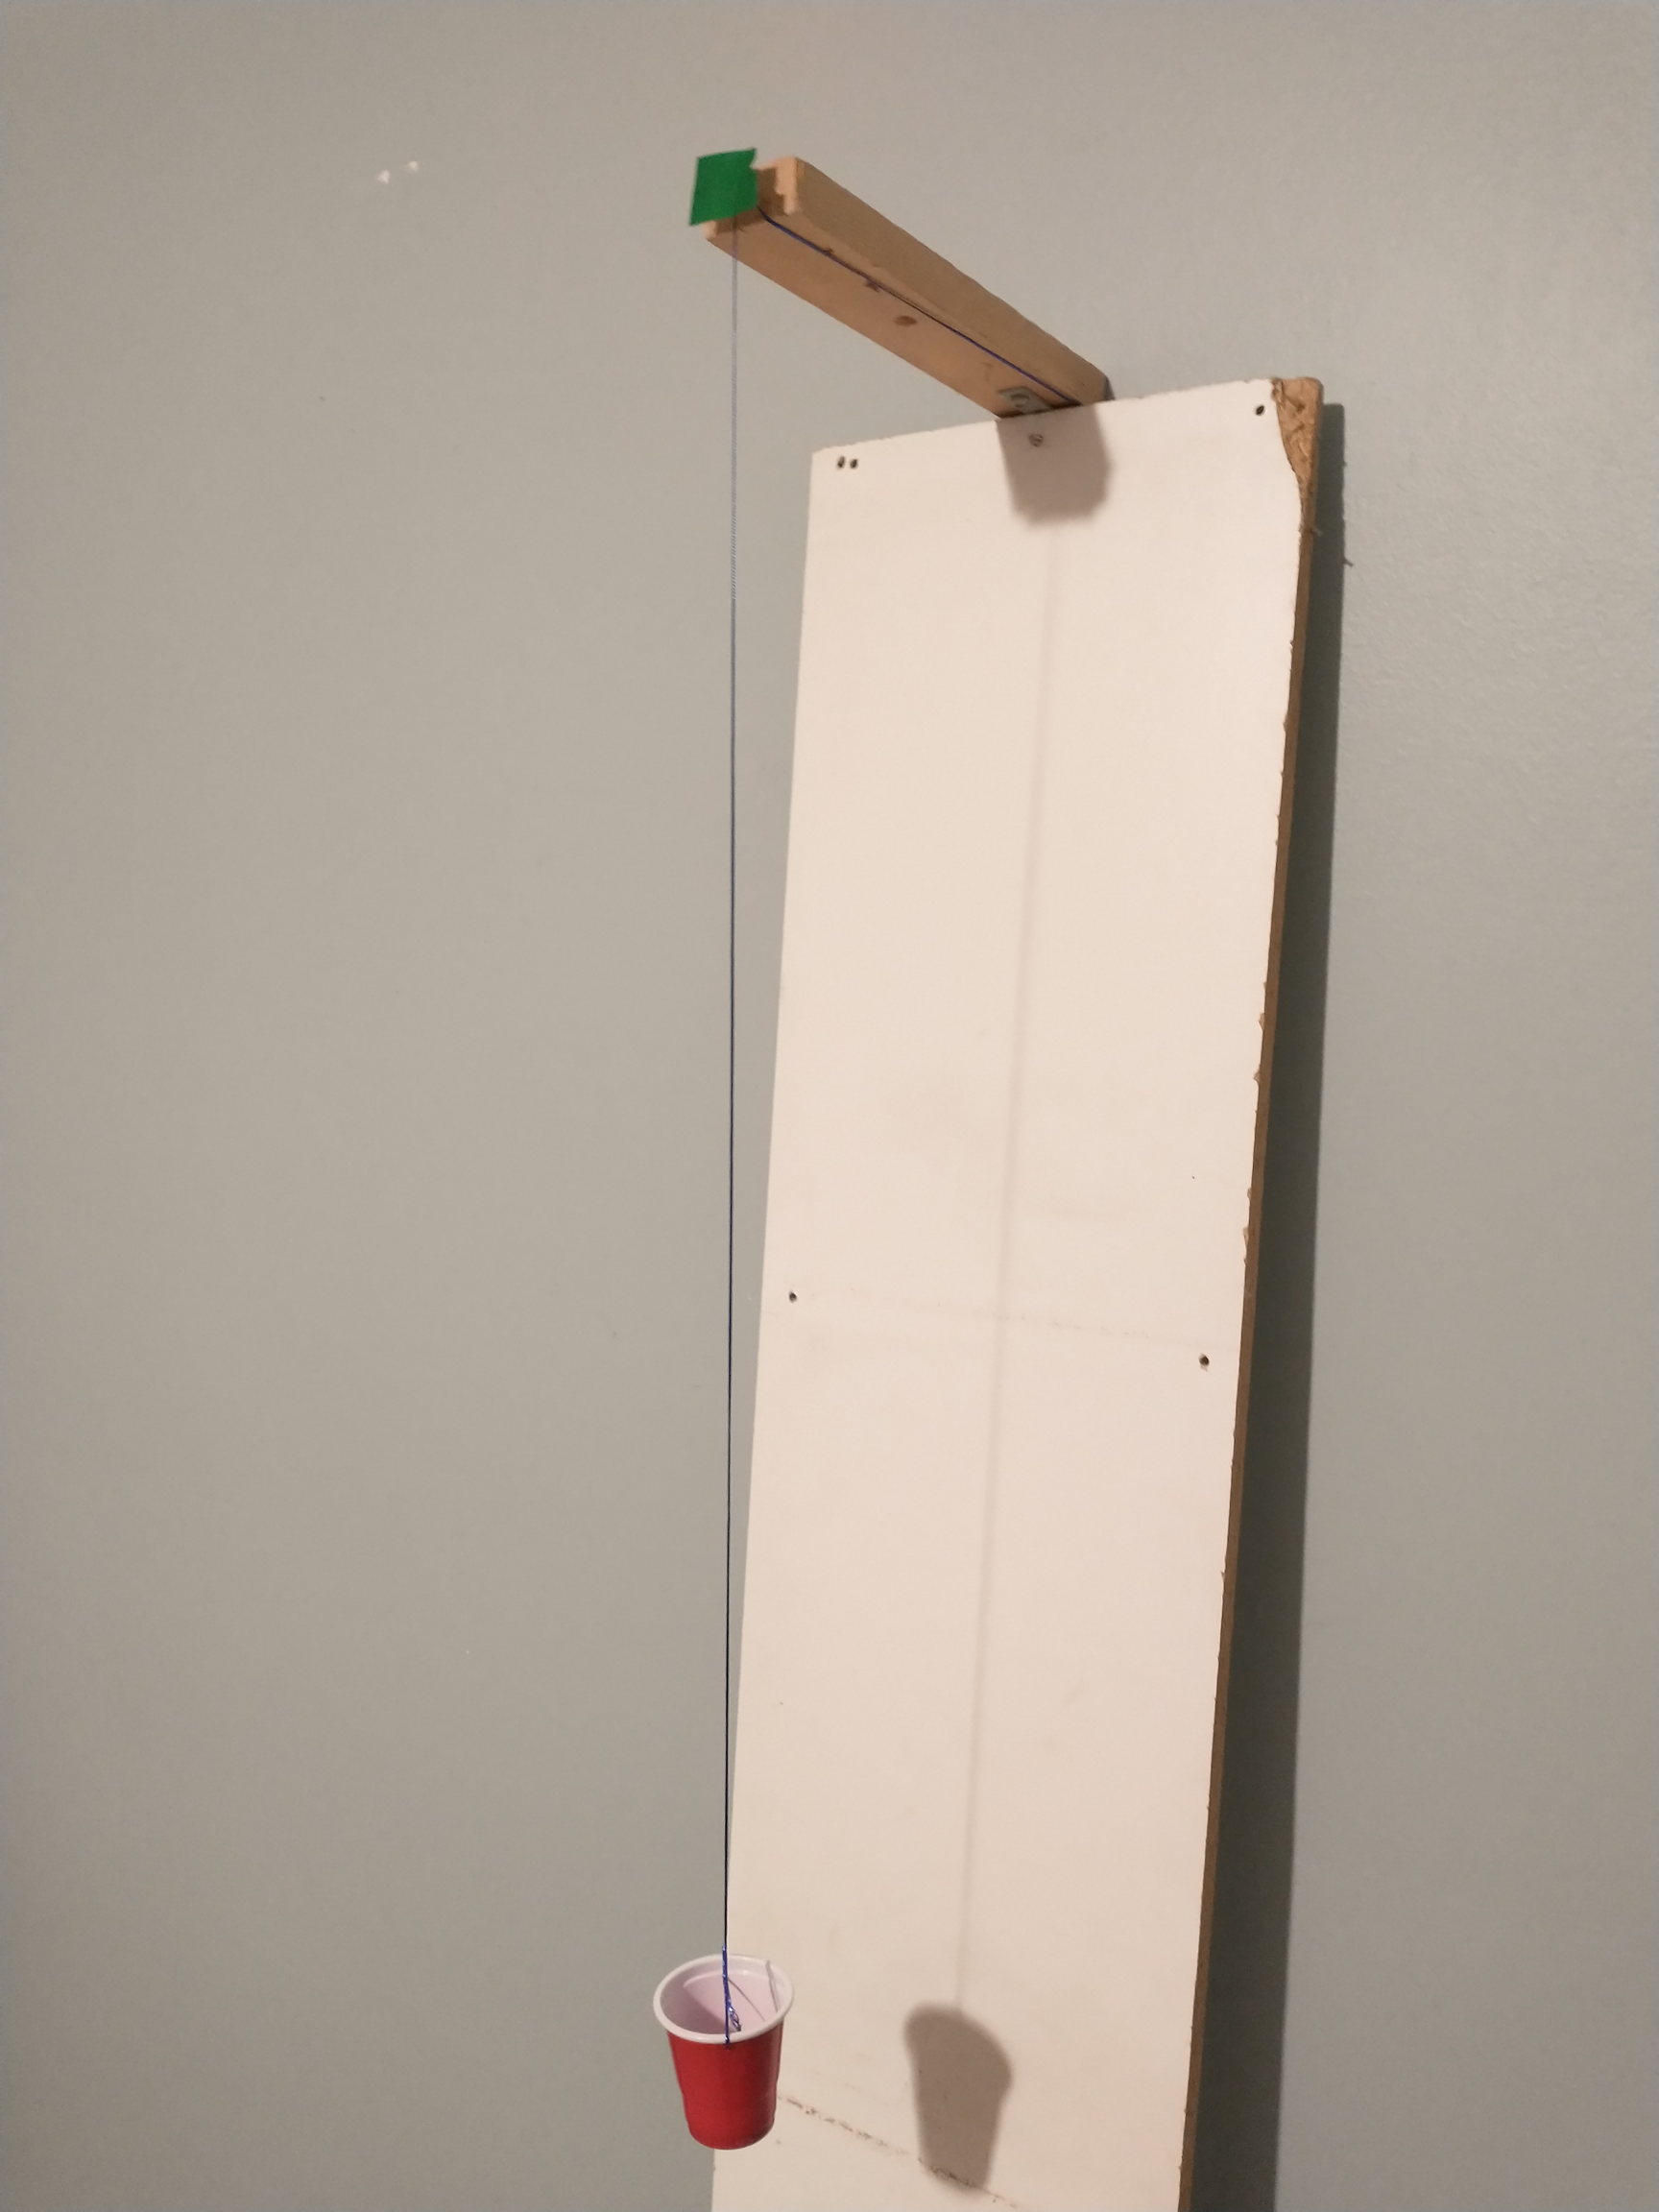
\includegraphics[width=0.6\linewidth]{pendulum.png}
    \caption{The pendulum constructed for this experiment.}
\end{figure}

The main support structure of the pendulum consists of two pieces of wood, attached together with screws and an
L-bracket. This was chosen because the material was readily available, and could be substituted for any material of
similar size and suitable strength.

The string of the pendulum is a thin, braided string, specifically chosen for visibility and to minimize twisting in
order to keep the motion of the pendulum in the same plane. The string is wound around a screw at the top, with a piece
of green reflective tape on it for tracking.

The string is attached to a bob consisting of a small, red plastic cup with coins inside for weight. The colour of the
cup is deliberately chosen to allow for computer-vision (CV) based tracking. Coins are used for added weight because
they have known masses and are readily available.

The string length and bob mass are adjustable, but for this experiment, the distance from the pivot to the centre of the
mass is fixed at \(65\si{cm} \pm 1\si{cm}\), and the mass is fixed at 6 Canadian \$2 coins (about \(41.52\si{g}\)
assuming cup mass is negligible).

\subsection{Data Collection}

\begin{figure}[htb]
    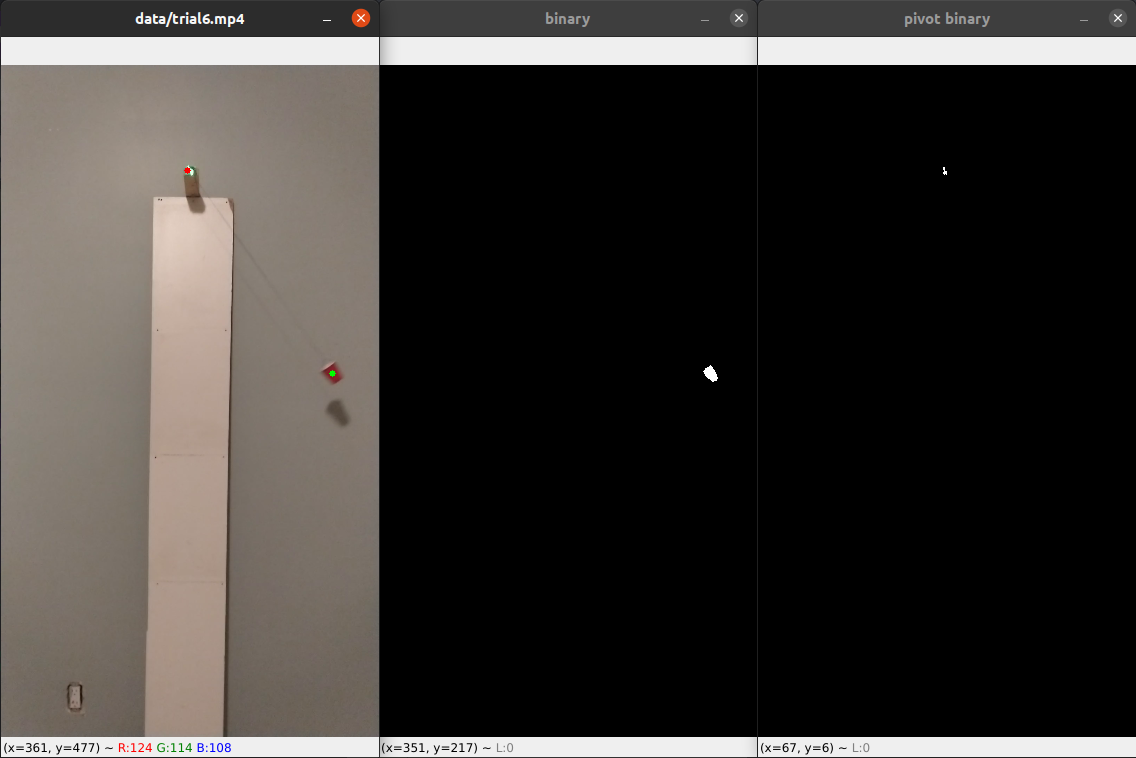
\includegraphics[width=\linewidth]{cv_track.png}
    \caption{CV-based tracking of the pendulum.}
\end{figure}

Videos of the pendulum are shot on a phone camera in FHD 60fps and then passed to a program to determine the angles.
The pendulum swings in the plane of the camera.

The pendulum's angle is tracked using a Python program written with OpenCV (see Appendix \ref{appendix:code}).
The locations of the bob and pivot are determined by thresholding the image and then taking the average of the pixels to
find the centres. After the pixel coordinates have been determined, the ratio of the difference between the \(x\) and
\(y\) coordinates are used to compute the angle for each frame.
One data point is collected per 3 frames for 20 data points per second.

\subsection{Data Analysis}

In total, 7 trials were conducted.
For each trial, the \(Q\) factor is determined using two independent methods as outlined below:

\subsubsection{Curve Fitting}

In the first method, \(Q\) is computed using Equation \ref{eqn:q} with values of \(\tau\) and \(T\) computed by fitting
Equation \ref{eqn:model} to the experimental data.

The data is passed to a Python program (see Appendix \ref{appendix:code}) that fits the model using a nonlinear
least-squares method, which determines the optimal values for \(\tau\) and \(T\) among others, and the standard
deviations of both, which is used as the uncertainty.

\subsubsection{Oscillation Counting}

In the second method, the number of oscillations until the amplitude decays to \(e^{-\pi/3}\) of the original is
counted, which corresponds to \(\frac{Q}{3}\). The counting is again done with a Python program (see Appendix
\ref{appendix:code}).

Note that here we define an "oscillation" as one complete period of the pendulum's swing. "Half-oscillations" are
counted if the amplitude first reaches the target value without completing a full period. For example, if the pendulum
starts at all the way to the right, and first reaches the target amplitude when it is swinging all the way to the left,
then a half-oscillation will be counted for the last cycle.

%%%%%%%%%%%%%%%%%%%%%%%%%%%%%%%%%%%%%%%%%%%%%%%%%%%%%%%%%%%%%%%%%%

\section{Observations}

\subsection{Curve Fitting}

\begin{figure*}[htb]
    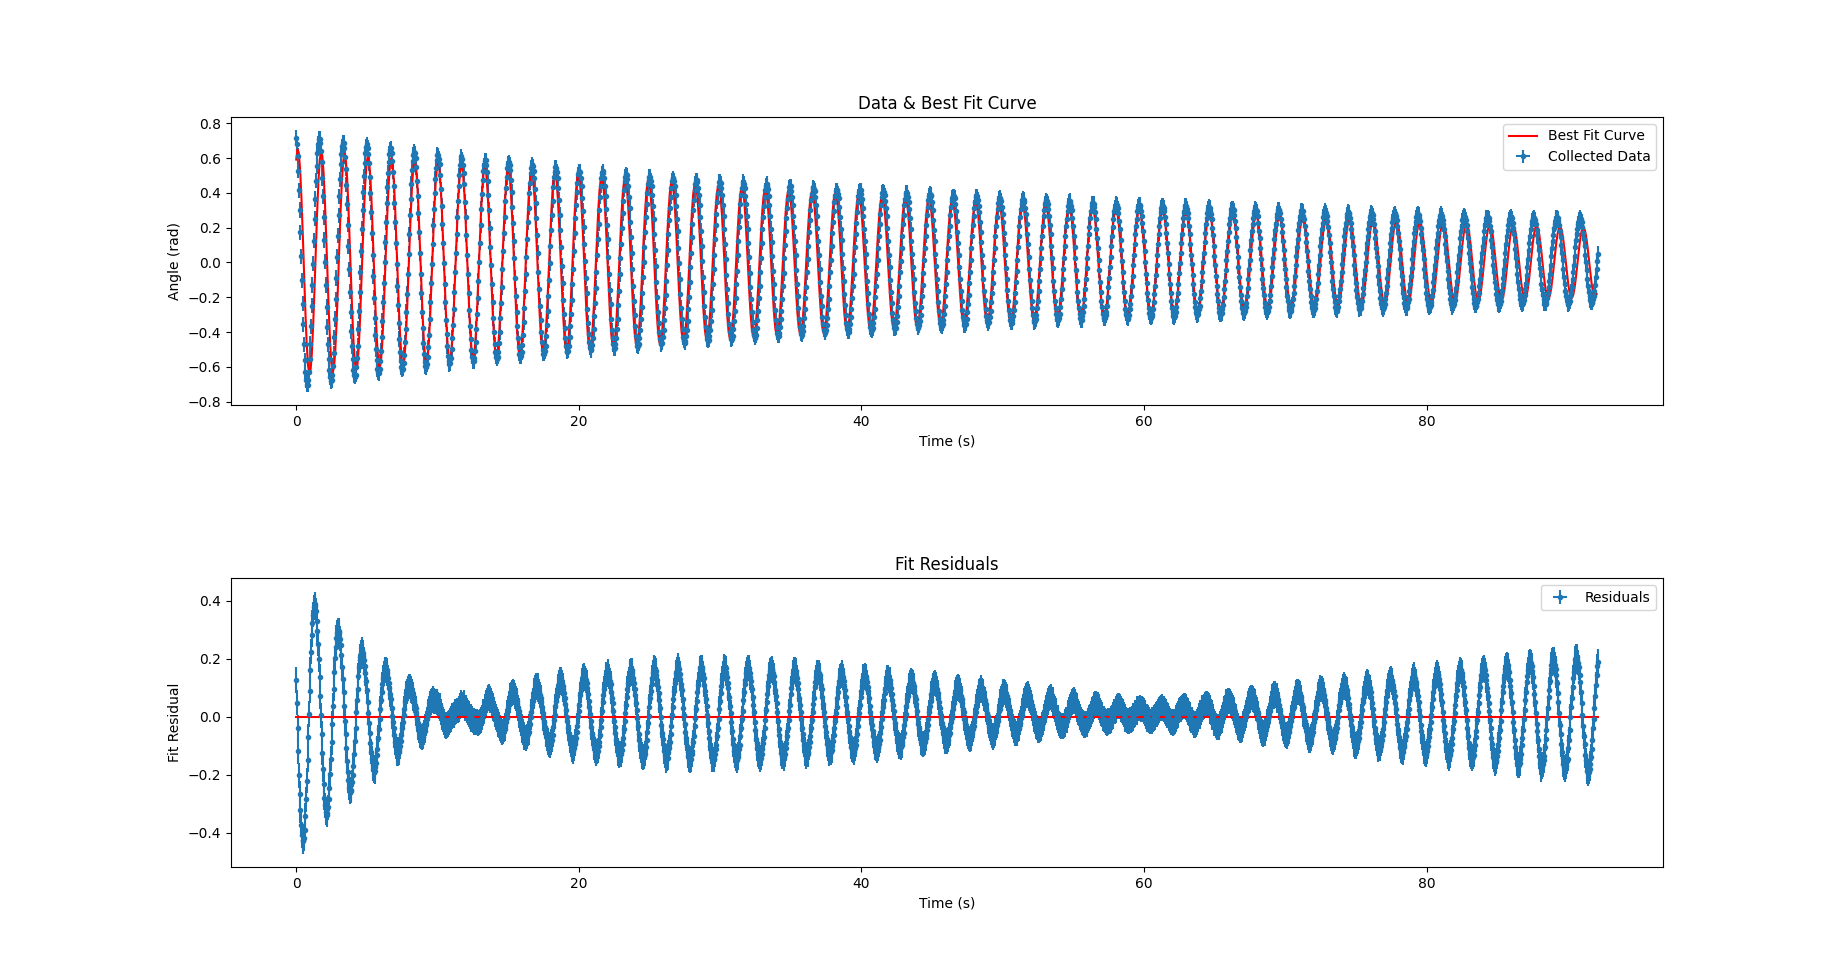
\includegraphics[width=\linewidth]{fit1.png}
    \caption{Result of fitting Equation \ref{eqn:model} to the data.}
    \label{fig:fit}
\end{figure*}
\begin{figure*}[htb]
    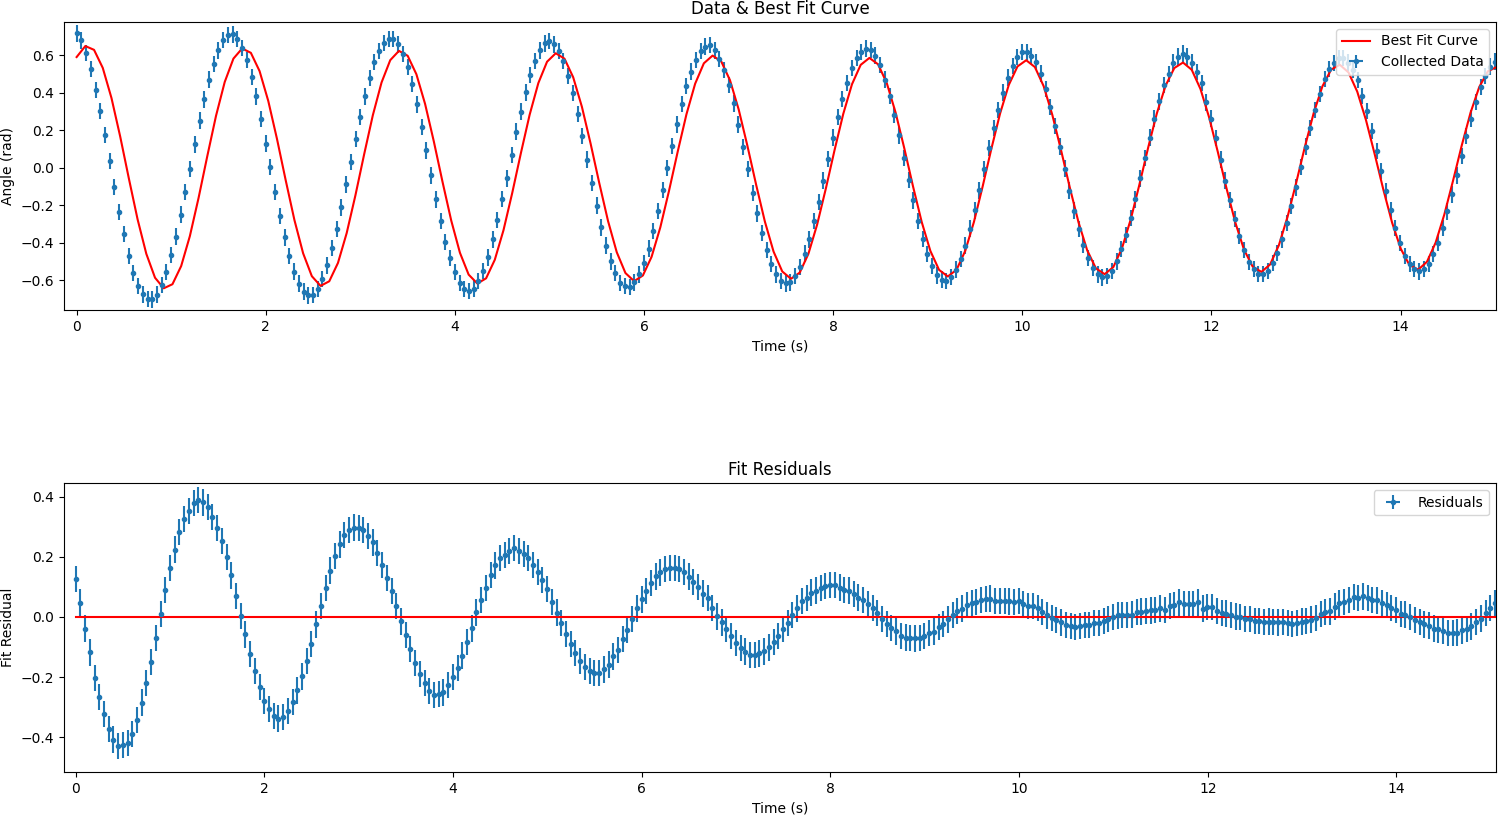
\includegraphics[width=\linewidth]{fit2.png}
    \caption{Zoomed in view of the first 15 seconds.}
    \label{fig:fitzoom}
\end{figure*}

\(Q\) values computed using this method are shown below:
\begin{table}[h]
    \begin{tabular}{ccc}
        Trial & \(Q\) & Uncertainty \\
        \hline
        1   & 153.49    & \(\pm 2.12\) \\
        2   & 147.89    & \(\pm 3.95\) \\
        3	& 140.96	& \(\pm 3.53\) \\
        4	& 151.12	& \(\pm 3.81\) \\
        5	& 130.24	& \(\pm 3.86\) \\
        6	& 131.31	& \(\pm 3.76\) \\
        7	& 138.04	& \(\pm 3.70\) \\
        \hline
        \multicolumn{2}{l}{Mean} & 141.86 \\
        \multicolumn{2}{l}{Standard Deviation} & 9.30 \\
        \multicolumn{2}{l}{Uncertainty of the Mean} & 3.52
    \end{tabular}
    \caption{Raw data from curve fitting; values are \textbf{unrounded}. For final uncertainties see Section
        \ref{section:uncertainty}. Note standard deviations use the \textit{sample} standard deviation formula.}
\end{table}

A graph of the data and curve fit for one trial is shown in Figure \ref{fig:fit} and Figure \ref{fig:fitzoom}.

\subsection{Oscillation Counting}

\(Q\) values computed using this method are shown below:
\begin{table}[h]
    \begin{tabular}{cc}
        Trial & \(Q\)\\
        \hline
        1   & 148.5 \\
        2   & 151.5 \\
        3	& 148.5 \\
        4	& 154.5 \\
        5	& 139.5 \\
        6	& 142.5 \\
        7	& 148.5 \\
        \hline
        \multicolumn{1}{l}{Mean} & 147.6 \\
        \multicolumn{1}{l}{Standard Deviation} & 5.11 \\
        \multicolumn{1}{l}{Uncertainty of the Mean} & 1.93
    \end{tabular}
    \caption{Raw data from oscillation counting. For uncertainties see Section \ref{section:uncertainty}}
\end{table}

It was chosen to measure for \(\frac{Q}{3} \implies e^{-\pi/3} \approx 0.3509\) because of the very high \(Q\) factor of
the pendulum. The data collected only covers a time range enough for \(\frac{Q}{3}\).

However, an interesting phenomenon can be observed by varying the fraction of \(Q\) to measure for.
For example, if we measure for \(\frac{Q}{4}\) instead, we get this data:
\begin{table}[h]
    \begin{tabular}{cc}
        Trial & \(Q\)\\
        \hline
        1   & 126.0 \\
        2   & 138.0 \\
        3	& 134.0 \\
        4	& 144.0 \\
        5	& 128.0 \\
        6	& 126.0 \\
        7	& 134.0 \\
        \hline
        \multicolumn{1}{l}{Mean} & 132.9 \\
        \multicolumn{1}{l}{Standard Deviation} & 6.72 \\
        \multicolumn{1}{l}{Uncertainty of the Mean} & 2.54
    \end{tabular}
\end{table}

After more trials, it can be observed that the value of \(Q\) observed through counting oscillations is dependent on the
fraction of \(Q\) that was measured for. Moreover, as the denominator increases, the observed \(Q\) value seems to
decrease, while according to the mathematical model the value of \(Q\) should be independent of the fraction measured.
This is likely because the model is not an accurate approximation of the actual system. (More details in Section
\ref{section:analysis}.)

\subsection{Uncertainty Analysis}
\label{section:uncertainty}

%%%%%%%%%%%%%%%%%%%%%%%%%%%%%%%%%%%%%%%%%%%%%%%%%%%%%%%%%%%%%%%%%%

\section{Analysis}
\label{section:analysis}

TODO Include sources of error, e.g. systematic bias in angle

%%%%%%%%%%%%%%%%%%%%%%%%%%%%%%%%%%%%%%%%%%%%%%%%%%%%%%%%%%%%%%%%%%

\appendix
\section{Source Code}

A comprehensive list of all source code can be found on GitHub at \url{https://github.com/tylertian123/phys180_lab},
in particular:
\label{appendix:code}
\begin{enumerate}
    \item For tracking the pendulum and generating time-angle data: \url{https://github.com/tylertian123/phys180_lab/blob/master/cvtrack.py}
    \item For fitting the model to experimental data: \url{https://github.com/tylertian123/phys180_lab/blob/master/fit.py}
    \item For measuring \(Q\) by counting oscillations: \url{https://github.com/tylertian123/phys180_lab/blob/master/find_q.py}
\end{enumerate}

\end{document}
